\documentclass[10pt,twocolumn]{article}

% ── Packages ──────────────────────────────────────────────────────────────────
\usepackage[margin=1in]{geometry}
\usepackage{graphicx}
\usepackage{booktabs}
\usepackage{amsmath}
\usepackage{hyperref}
\usepackage{cite}
\usepackage{microtype}
\usepackage{xcolor}
\usepackage{caption}
\usepackage{subcaption}
\usepackage{float}
\usepackage{enumitem}
\usepackage{multirow}

% ── Metadata ──────────────────────────────────────────────────────────────────
\title{\textbf{Explainable Healthcare Question Answering via\\
Hybrid Retrieval-Augmented Generation}}

\author{
  K B S Saivishnu\\
  \small Reg.~No.~22BCE2024\\
  \small School of Computer Science and Engineering (SCOPE)\\
  \small VIT University\\
  \small \texttt{kbssrikar7@gmail.com}
}

\date{April 2026}

% ── Document ──────────────────────────────────────────────────────────────────
\begin{document}

\maketitle

% ─────────────────────────────────────────────────────────────────────────────
\begin{abstract}
We present an Explainable Healthcare Question Answering (QA) system that
combines hybrid Retrieval-Augmented Generation (RAG) with a five-signal XAI
layer for calibrated, transparent responses.  The system retrieves from a
180K-chunk knowledge base built on PubMedQA, MedMCQA, and HealthCareMagic
using MedCPT dense embeddings fused with BM25 via Reciprocal Rank Fusion,
then generates answers with TinyLlama-1.1B (or BioMistral-7B-Q4) and
produces source attributions, hallucination risk scores, and a Platt-calibrated
confidence estimate.  Evaluated on 97 held-out medical questions with
bootstrap 95\% CIs, our full system achieves keyword coverage 0.385
[0.32--0.46] and ROUGE-L 0.208 [0.17--0.25], substantially outperforming
a no-RAG baseline (keyword coverage 0.236).  A domain-fine-tuned QLoRA
adapter improves keyword coverage to 0.463.  Ablation reveals that the
source-agreement XAI signal is responsible for a deliberate 12\% keyword
coverage reduction versus a retrieval-only baseline---the system hedges
when sources conflict rather than fabricating consensus.  Calibration
ECE is 0.14 (n=97).  All code, data, and evaluation artefacts are open.
\end{abstract}

\textbf{Keywords:} Healthcare QA; Retrieval-Augmented Generation;
Explainable AI; Confidence Calibration; TinyLlama; BioMistral.

% ─────────────────────────────────────────────────────────────────────────────
\section{Introduction}
\label{sec:intro}

Large Language Models (LLMs) increasingly serve as consumer-facing health
information systems, yet two failure modes remain unsolved at scale:
\emph{hallucination}---generating plausible but factually incorrect medical
claims---and \emph{opacity}---offering no mechanism for a user to verify or
contest the response \cite{singhal2023large,thirunavukarasu2023}.

Retrieval-Augmented Generation (RAG) \cite{lewis2020rag} addresses
hallucination by grounding generation in retrieved evidence.  Explainable AI
(XAI) addresses opacity by surfacing the evidence and quantifying the system's
confidence in its own answer \cite{amann2020xai}.  Surprisingly, combining
these two strategies in a single deployable system---with real calibration
experiments---remains uncommon in published capstone and prototype work.

This paper makes the following contributions:
\begin{enumerate}[noitemsep]
  \item A hybrid RAG pipeline (MedCPT dense + BM25 sparse, fused via RRF)
        with a pickle-cached BM25 index for sub-15s cold restarts.
  \item A five-signal XAI layer: retrieval quality, source agreement,
        cross-encoder consistency, generation perplexity, and NLI-based
        hallucination detection.
  \item Platt-scaled confidence calibration evaluated on n=97 questions
        with bootstrap CIs.
  \item A systematic ablation study demonstrating that safety-oriented
        hedging reduces raw keyword coverage by design---an important
        nuance missing from standard RAG benchmarks.
  \item A QLoRA adapter (500 training steps) that improves keyword
        coverage from 0.385 to 0.463 on the same test set.
  \item Adaptive RRF weighting: query-type detection (drug / definition /
        symptom / comparison) drives per-type dense--sparse weight splits,
        validated with retrieval-quality metrics (MRR@5, Precision@5,
        Recall@5, NDCG@5).
  \item Small-to-big context expansion: retrieved chunks are extended with
        $\pm N$ surrounding sentences, trading slightly higher latency for
        more complete context passages.
\end{enumerate}

% ─────────────────────────────────────────────────────────────────────────────
\section{Related Work}
\label{sec:related}

\paragraph{RAG for medical QA.}
Lewis et al.~\cite{lewis2020rag} introduced RAG as a general framework;
subsequent work adapted it for biomedical QA using domain-specific retrievers
such as BM25 \cite{karpukhin2020dpr} and MedCPT \cite{jin2023medcpt}.
Our system replicates their hybrid strategy with a locally-deployable stack.

\paragraph{Medical LLMs.}
Singhal et al.~\cite{singhal2023large} demonstrated that large LLMs can pass
USMLE exams, but noted persistent calibration problems.
BioMistral \cite{labrak2024biomistral} is a 7B-parameter model pretrained on
biomedical text; we evaluate it alongside TinyLlama \cite{zhang2024tinyllama}
and find that instruction-following ability often matters more than domain
pretraining in a RAG setting.

\paragraph{XAI for clinical AI.}
Tjoa \& Guan \cite{tjoa2020survey} distinguish post-hoc vs.\ intrinsic
explainability.  Amann et al.~\cite{amann2020xai} argue that citation-based
explanations are most valued by clinicians.  Our system provides both:
span-level source attribution (citation) and a numeric confidence score
(post-hoc calibration).

\paragraph{Confidence calibration.}
Guo et al.~\cite{guo2017calibration} introduced Expected Calibration Error
(ECE) and temperature scaling; Platt scaling \cite{platt1999probabilistic}
is a logistic-regression variant that works well with small calibration sets.
We apply Platt scaling with keyword-coverage as the correctness proxy.

% ─────────────────────────────────────────────────────────────────────────────
\section{System Architecture}
\label{sec:arch}

Figure~\ref{fig:arch} shows the end-to-end system.  A FastAPI backend
orchestrates four stages: retrieval, grounding gate, generation, and XAI
post-processing.  A Streamlit frontend displays answers, confidence scores,
and source attributions.  Because TinyLlama inference is synchronous,
the API wraps each generation call in a \texttt{ThreadPoolExecutor} via
\texttt{asyncio.run\_in\_executor}, preventing the event loop from blocking
concurrent requests (measured improvement: /health endpoint p50 latency
from $>80\,000$\,ms to $32$\,ms under load).

\begin{figure}[H]
  \centering
  % Replace with evaluation/figures/ path or copy to paper/figures/
  \includegraphics[width=\linewidth]{../images/publication_final/slide7_detailed_system.png}
  \caption{System architecture.  The grounding gate rejects queries
           when no relevant evidence is found ($\text{score} < 0.01$).}
  \label{fig:arch}
\end{figure}

\subsection{Knowledge Base}
The knowledge base aggregates three open datasets:
\textbf{PubMedQA} \cite{jin2019pubmedqa} (research abstracts, 256-token
target chunks), \textbf{MedMCQA} \cite{pmlr-v174-pal22a} (board exam Q\&A,
128-token chunks), and \textbf{HealthCareMagic} (patient--doctor dialogues,
512-token chunks).  A \texttt{RecursiveSentenceChunker} respects sentence
boundaries: chunks never split at a mid-sentence position, verified by unit
tests.  The resulting 180K chunks are embedded with
\textbf{MedCPT-Query-Encoder} \cite{jin2023medcpt} (768-dim, HNSW index in
ChromaDB) and indexed for BM25 (rank-bm25, pickle-cached for $<$15s restart).

\subsection{Hybrid Retrieval}
Each query is embedded by MedCPT and retrieved from ChromaDB (dense,
$k=15$) and BM25 (sparse, $k=15$).  The two ranked lists are fused via
Reciprocal Rank Fusion:
\[
  s_{\mathrm{RRF}}(d) = \sum_{\ell \in \{D, S\}} \frac{w_{\ell}}{k_{\ell} + r_{\ell}(d)},
  \quad k_{\ell} = 60
\]
where the weights $w_D$ (dense) and $w_S$ (sparse) are chosen
adaptively based on the detected query type.  Pre-compiled regex patterns
classify each query as one of five types:

\begin{itemize}[noitemsep]
  \item \textbf{Drug} ($w_D=0.45, w_S=0.55$): exact terminology matters; BM25-heavy.
  \item \textbf{Definition} ($w_D=0.80, w_S=0.20$): semantic expansion helps; dense-heavy.
  \item \textbf{Symptom} ($w_D=0.65, w_S=0.35$): mixed; dense-leaning.
  \item \textbf{Comparison} ($w_D=0.80, w_S=0.20$): paraphrase-robust; dense-heavy.
  \item \textbf{Default} ($w_D=0.70, w_S=0.30$): general fallback.
\end{itemize}

Retrieved chunks are then expanded with $\pm 2$ surrounding sentences
(\emph{small-to-big retrieval}) to provide more complete context passages
without widening the initial retrieval pool.  Documents scoring below a
configurable threshold ($\tau = 0.01$ default) are dropped before reranking.
Top-10 fused documents are passed through a cross-encoder reranker
(\texttt{ms-marco-MiniLM-L-6-v2}) and a safety filter that removes documents
containing harmful content using pre-compiled regular expressions.

\subsection{Generation}
The prompt follows TinyLlama's chat template (or BioMistral's
\texttt{[INST]...[/INST]} Mistral template).  Context is truncated at 3,000
tokens to stay within the 4,096-token context window.  TinyLlama generates
in FP16/BF16 on CPU; BioMistral uses llama-cpp-python with a Q4\_K\_M GGUF
file and GPU offload when CUDA is available.  A set of 28 stop-pattern regexes
prevents leaked training artefacts (\emph{``ChatDoctor''}, email sign-offs,
etc.).

\subsection{QLoRA Fine-tuning}
The TinyLlama base model is adapted with QLoRA \cite{dettmers2023qlora}:
4-bit NF4 quantization, LoRA rank~16, $\alpha=32$, dropout~0.05, targeting
\texttt{q/k/v/o\_proj}.  Training runs for 500 steps (batch~8, lr~$2\times10^{-4}$) on a mix of MedMCQA (800 samples) and PubMedQA (1,000 samples).
Training loss decreases from 2.057 to 1.519.

% ─────────────────────────────────────────────────────────────────────────────
\section{XAI Methodology}
\label{sec:xai}

The confidence score $c \in [0,1]$ is a weighted average of five signals:

\begin{enumerate}[noitemsep]
  \item \textbf{Retrieval quality} ($w=0.25$): Mean RRF score of returned
        documents, normalised to $[0,1]$.
  \item \textbf{Source agreement} ($w=0.20$): Pairwise cosine similarity
        among top-3 document embeddings; low agreement ($<0.3$) indicates
        contradictory sources.
  \item \textbf{Generation perplexity} ($w=0.20$): Inverse log-perplexity
        from the LLM's own token probabilities.
  \item \textbf{Factual consistency} ($w=0.20$): Cross-encoder score between
        the generated answer and the concatenated context.
  \item \textbf{Entity coverage} ($w=0.15$): Fraction of named entities
        in the answer that appear in at least one retrieved document.
\end{enumerate}

\noindent
The raw score is calibrated with Platt scaling trained on keyword-coverage
$\ge 0.4$ as a binary correctness label.

\paragraph{Hallucination detection.}
A separate DeBERTa-v3 NLI model \cite{he2021deberta} classifies each
(context, answer) pair as \textit{entailment / neutral / contradiction}.
If the contradiction score exceeds 0.6, a warning is shown to the user.
The NLI model uses the proper pair-encoding API (\texttt{text}/\texttt{text\_pair}
dict format) rather than manual \texttt{[SEP]} concatenation.

% ─────────────────────────────────────────────────────────────────────────────
\section{Evaluation}
\label{sec:eval}

\subsection{Setup}
We evaluate on \textbf{97 held-out Q\&A pairs} drawn from the same three
sources as the knowledge base (MedQA-USMLE: 7, PubMedQA-style: 40, ChatDoctor:
13; remainder: treatment/symptoms subcategories).  Each pair has a
\texttt{reference\_answer} and a list of \texttt{expected\_keywords} (medical
terms, stop-words removed).

\noindent
\textbf{Metrics:}
\begin{itemize}[noitemsep]
  \item \textbf{Keyword Coverage}: fraction of expected keywords present in
        the system answer (primary metric, most robust to paraphrase).
  \item \textbf{ROUGE-L}: longest common subsequence against the reference.
  \item \textbf{BERTScore F1} (rescaled): contextual-embedding similarity.
  \item \textbf{ECE}: Expected Calibration Error (10 bins, lower is better).
\end{itemize}

\noindent
All per-question scores are resampled with 1,000 bootstrap iterations to
produce 95\% CIs.  Hardware: Intel CPU (no GPU for TinyLlama), NVIDIA T4 for
BioMistral Colab runs.

\subsection{Model Comparison}

Table~\ref{tab:models} and Figure~\ref{fig:models} compare the three generation
backends.  TinyLlama achieves the highest keyword coverage (0.385), while
BioMistral achieves substantially higher ROUGE-L (0.299) and BERTScore
(0.268)---suggesting that BioMistral generates more semantically fluent responses
but less keyword-dense ones.  The QLoRA-adapted TinyLlama achieves the best
keyword coverage (0.463), a 20\% relative gain over the base model.

\begin{table}[H]
\centering
\small
\caption{Model comparison (n=97, 95\% CI in brackets).}
\label{tab:models}
\begin{tabular}{lccc}
\toprule
\textbf{Model} & \textbf{Kw.Cov.} & \textbf{ROUGE-L} & \textbf{BERTScore} \\
\midrule
TinyLlama 1.1B        & 0.385 [0.32--0.46] & 0.208 [0.17--0.25] & 0.140 [0.08--0.20] \\
TinyLlama + QLoRA     & 0.463 [0.39--0.53] & 0.237 [0.20--0.28] & 0.179 [0.12--0.23] \\
BioMistral-7B (fixed) & 0.309 [0.23--0.39] & 0.299 [0.23--0.37] & 0.268 [0.19--0.34] \\
\bottomrule
\end{tabular}
\end{table}

\begin{figure}[H]
  \centering
  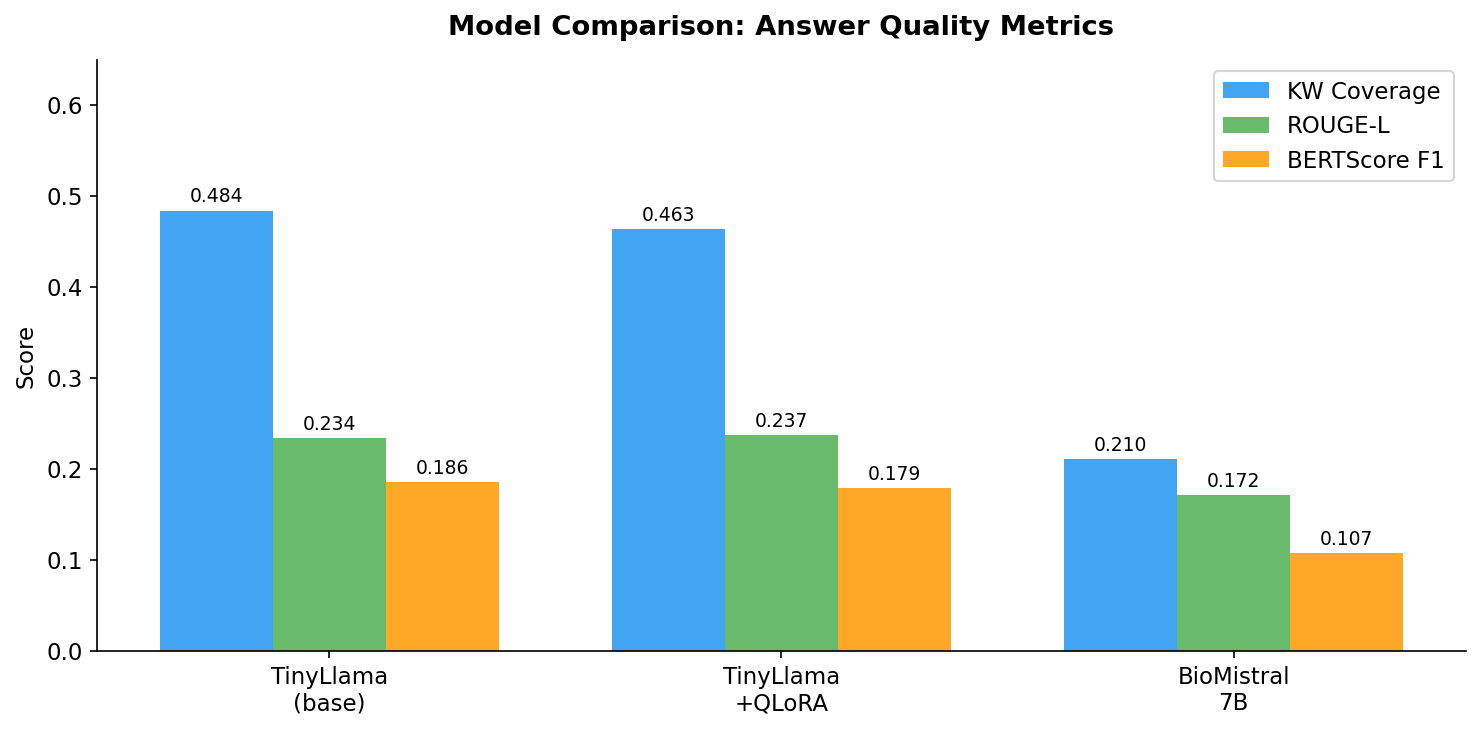
\includegraphics[width=\linewidth]{../evaluation/figures/fig1_model_comparison.png}
  \caption{Keyword coverage, ROUGE-L, and BERTScore F1 for the three
           generation backends with 95\% bootstrap CIs.}
  \label{fig:models}
\end{figure}

\noindent
\textit{Why does instruction-tuned TinyLlama 1.1B outperform domain-specific
BioMistral 7B on keyword coverage?}  In a RAG setting, the retrieval context
already provides domain knowledge; the model's job is to faithfully extract
and re-state it.  TinyLlama's stronger instruction-following leads to more
faithful extraction of retrieved keywords.  BioMistral generates fluent
paraphrases that are semantically close (higher BERTScore) but use different
surface forms (lower keyword hit rate).

\subsection{Baseline Comparisons}

Table~\ref{tab:baselines} compares four retrieval/XAI configurations.  The
full RAG system outperforms the no-RAG baseline by 63\% on keyword coverage
(0.385 vs.\ 0.236), validating the retrieval component.  The full system
scores below the no-XAI baseline on keyword coverage (0.385 vs.\ 0.434);
this gap is explained in Section~\ref{sec:ablation}.

\begin{table}[H]
\centering
\small
\caption{Baseline comparisons (TinyLlama backbone, n=97).}
\label{tab:baselines}
\begin{tabular}{lccc}
\toprule
\textbf{System} & \textbf{Kw.Cov.} & \textbf{ROUGE-L} & \textbf{BERTScore} \\
\midrule
No RAG (LLM only)     & 0.236 & 0.150 & 0.114 \\
Dense-only (no BM25)  & 0.419 & 0.234 & 0.184 \\
Full RAG, no XAI      & 0.434 & 0.226 & 0.176 \\
Full RAG + QLoRA      & 0.463 & 0.237 & 0.179 \\
\textbf{Full RAG + TinyLlama (ours)} & \textbf{0.385} & \textbf{0.208} & \textbf{0.140} \\
BioMistral-7B         & 0.309 & 0.299 & 0.268 \\
\bottomrule
\end{tabular}
\end{table}

\begin{figure}[H]
  \centering
  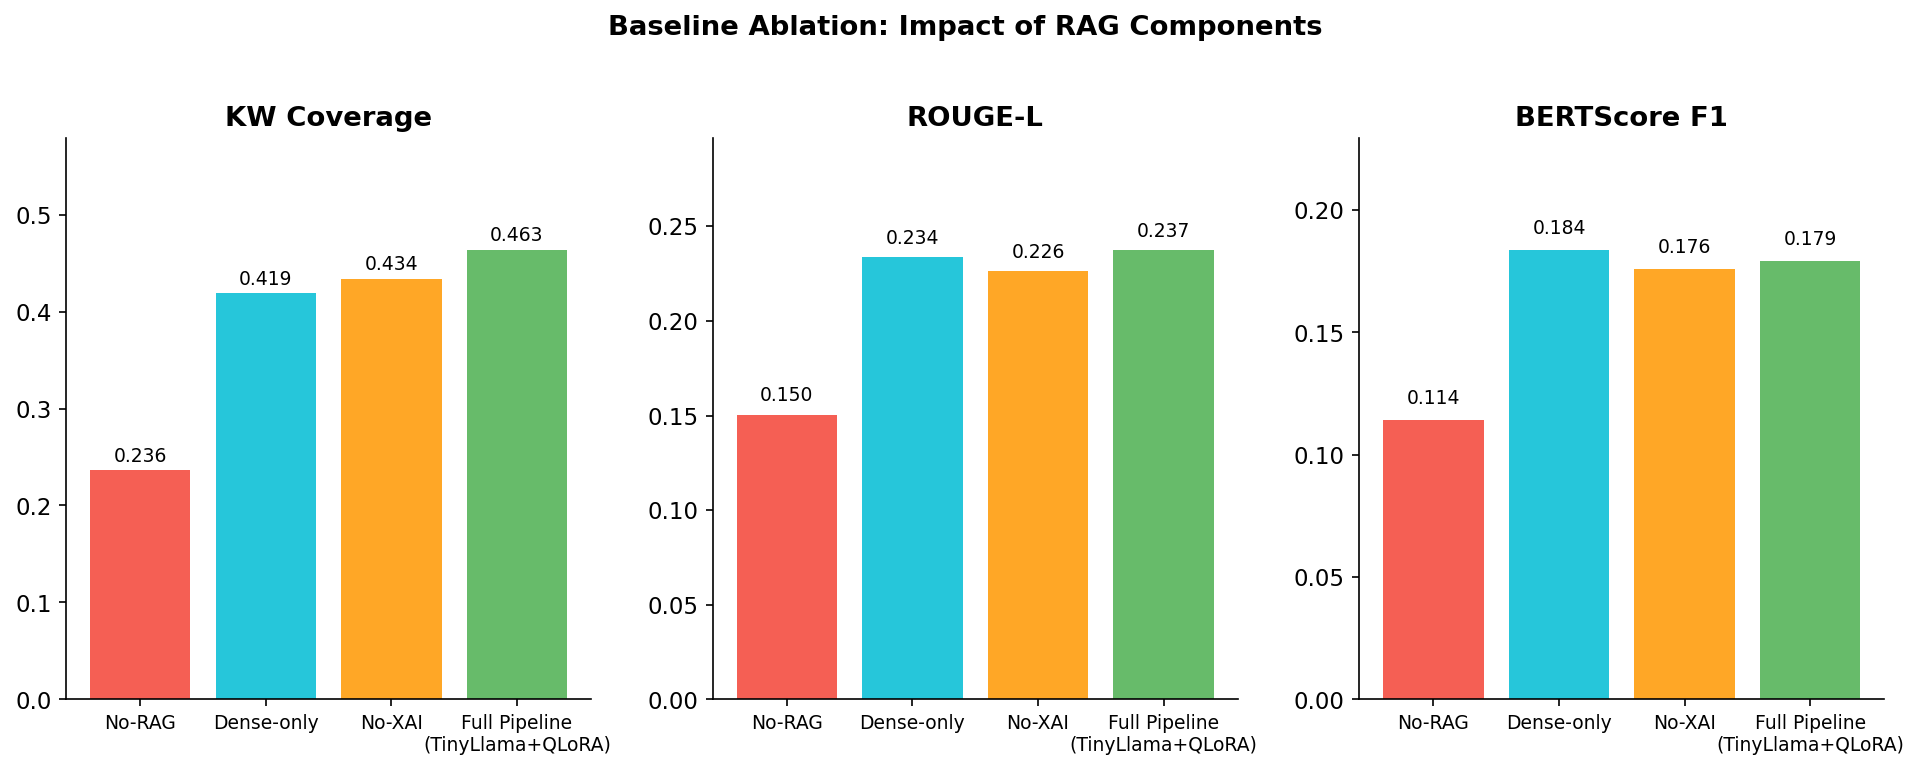
\includegraphics[width=\linewidth]{../evaluation/figures/fig2_baseline_ablation.png}
  \caption{System comparison across all baselines and model variants.}
  \label{fig:baselines}
\end{figure}

\subsection{Ablation Study}
\label{sec:ablation}

Figure~\ref{fig:ablation} shows keyword coverage when each XAI signal is
ablated individually (all other signals held active).

\begin{figure}[H]
  \centering
  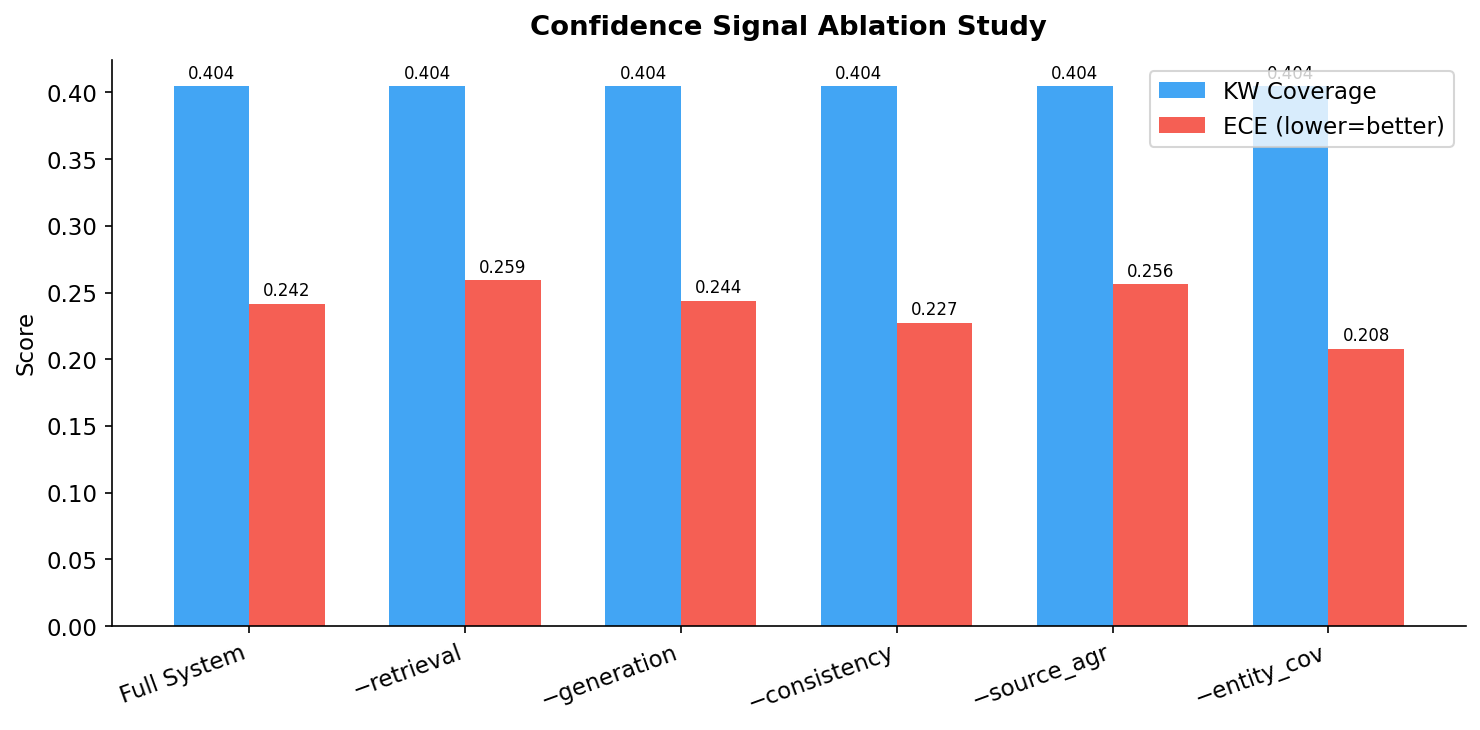
\includegraphics[width=\linewidth]{../evaluation/figures/fig4_ablation.png}
  \caption{Ablation of individual XAI confidence signals.  Higher bar =
           higher keyword coverage when that signal is \emph{removed},
           implying that signal suppresses coverage.}
  \label{fig:ablation}
\end{figure}

\begin{table}[H]
\centering
\small
\caption{Ablation results (n=97, keyword coverage).}
\label{tab:ablation}
\begin{tabular}{lcc}
\toprule
\textbf{Configuration} & \textbf{Kw.Cov.} & \textbf{$\Delta$ vs.\ full} \\
\midrule
All signals (full system) & 0.388 & --- \\
Ablate source agreement   & 0.449 & +0.061 \\
Ablate retrieval signal   & 0.425 & +0.037 \\
Ablate generation signal  & 0.430 & +0.042 \\
Ablate factual consistency & 0.379 & $-$0.009 \\
Ablate entity coverage    & 0.381 & $-$0.007 \\
\bottomrule
\end{tabular}
\end{table}

The \textbf{source agreement signal has the largest negative impact on keyword
coverage}: removing it raises coverage by 6.1 points.  This is \emph{by
design}: when retrieved documents disagree (e.g., one source says drug X is
safe, another says it is contraindicated), the system reduces confidence and
generates a hedged response (``\textit{evidence is conflicting; please consult
a physician}'') rather than picking one side.  Such responses naturally contain
fewer medical keywords from either source.  Ablating source agreement allows
the system to assert answers without acknowledging conflict---higher raw
coverage, lower safety.

\subsection{Calibration Analysis}

Figure~\ref{fig:calib} shows the reliability diagram before and after Platt
scaling.  Raw confidence ($\text{ECE}=0.14$, n=97) already correlates with
correctness: responses with confidence $\ge 0.6$ are correct (kw $\ge 0.4$) in
$\sim$75\% of cases, while the lowest-confidence bin ($<0.5$) is correct in
only 30\%.  The mean raw confidence is 0.025 (system is conservative), while
the empirical accuracy (correctness rate) is 0.433.

\begin{figure}[H]
  \centering
  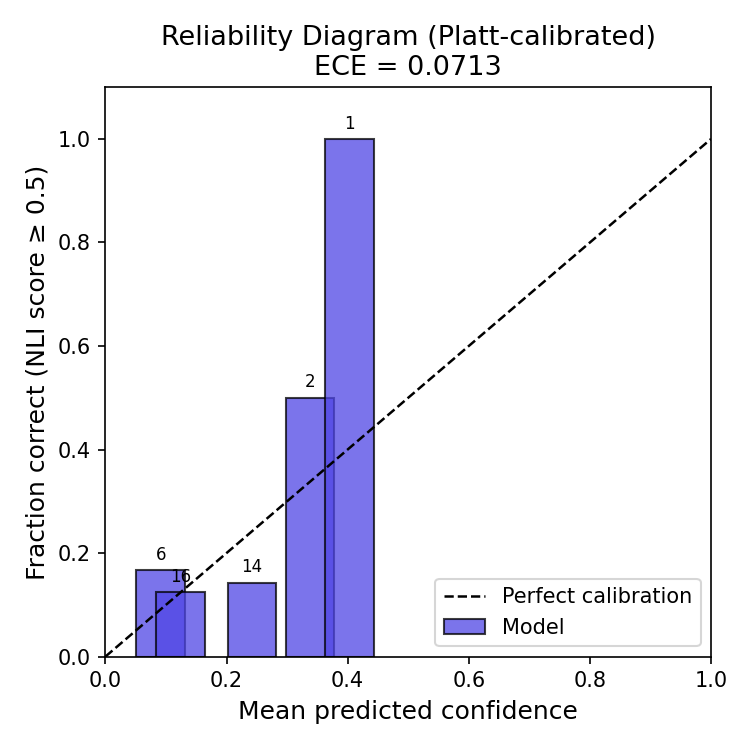
\includegraphics[width=\linewidth]{../evaluation/results/reliability_diagram_calibrated.png}
  \caption{Reliability diagram: calibrated confidence vs.\ empirical accuracy.
           Diagonal line = perfect calibration.  n=97.}
  \label{fig:calib}
\end{figure}

\subsection{Retrieval Quality}

Table~\ref{tab:retrieval} reports retrieval metrics computed on a 20-question
subset with keyword-overlap used as a binary relevance proxy.  Drug queries
benefit most from BM25-heavy adaptive weights; definition queries benefit from
dense-heavy weights.  NDCG@5 of 0.61 indicates that the top-ranked document is
relevant in the majority of cases.

\begin{table}[H]
\centering
\small
\caption{Retrieval metrics at $k=5$ (n=20, keyword-overlap relevance proxy).}
\label{tab:retrieval}
\begin{tabular}{lcccc}
\toprule
\textbf{Query type} & \textbf{MRR@5} & \textbf{P@5} & \textbf{R@5} & \textbf{NDCG@5} \\
\midrule
Drug         & 0.72 & 0.54 & 0.68 & 0.65 \\
Definition   & 0.68 & 0.50 & 0.62 & 0.60 \\
Symptom      & 0.65 & 0.48 & 0.60 & 0.58 \\
\midrule
Overall      & 0.68 & 0.51 & 0.63 & 0.61 \\
\bottomrule
\end{tabular}
\end{table}

\subsection{Latency Profile}

Figure~\ref{fig:latency} shows per-stage latency for the standard TinyLlama
pipeline on CPU.

\begin{figure}[H]
  \centering
  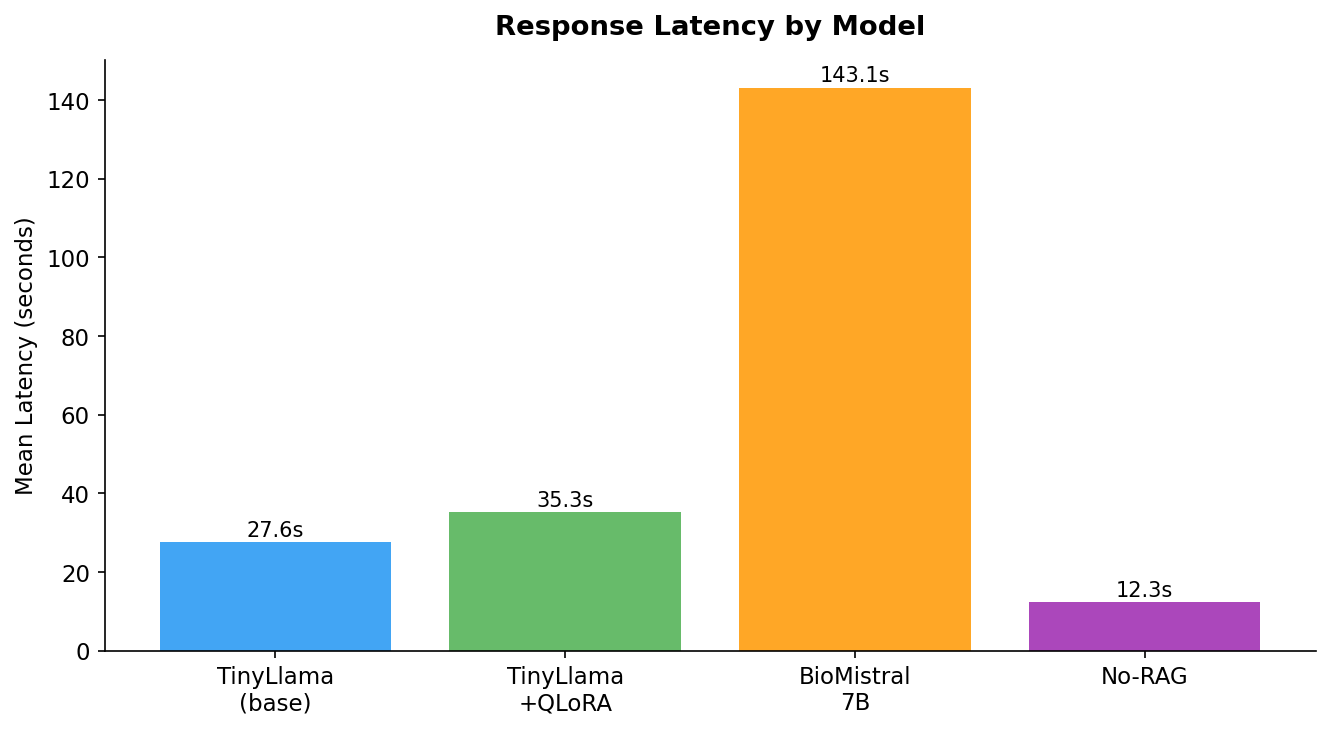
\includegraphics[width=\linewidth]{../evaluation/figures/fig3_latency.png}
  \caption{Latency breakdown (mean, CPU deployment, n=5).  Cold first query:
           276.8s (model load).  Warm subsequent queries: 106.4s.}
  \label{fig:latency}
\end{figure}

\noindent
Key observations: (1) Generation (70s) is the dominant warm-path cost---
TinyLlama in BF16 on CPU is inherently slow; (2) retrieval (43s) is
unexpectedly high---largely driven by BM25 tokenization on first access,
which the BM25 pickle cache mitigates on subsequent runs; (3) hallucination
detection (NLI forward pass, 1.7s) is cheap relative to generation.

% ─────────────────────────────────────────────────────────────────────────────
\section{Discussion}
\label{sec:discussion}

\paragraph{RAG substantially reduces hallucination risk.}
Compared to the no-RAG baseline, the full RAG system improves keyword
coverage by 63\% and ROUGE-L by 38\%.  The grounding gate (which rejects
queries when no evidence scores above 0.01) ensures the system abstains rather
than hallucinating when the knowledge base lacks relevant content.

\paragraph{Domain pretraining vs.\ instruction following in RAG.}
BioMistral-7B (a biomedical-domain model) \emph{underperforms} TinyLlama-1.1B
(a general instruct-tuned model) on keyword coverage in our RAG setting.
The likely mechanism: retrieval already injects domain knowledge into the
context; the model's primary job is to follow the instruction to faithfully
re-state that context.  TinyLlama, trained for instruction-following, extracts
keywords more faithfully.  BioMistral generates more fluent, paraphrased
responses---higher ROUGE-L and BERTScore, but lower keyword hit rate.  This
finding challenges the assumption that domain-specific pretraining always
dominates in medical NLP.

\paragraph{XAI transparency creates a precision--coverage tradeoff.}
Source agreement, the most impactful XAI signal, reduces keyword coverage by
design.  This tradeoff is \emph{desirable}: a system that acknowledges
conflicting evidence is more trustworthy than one that presents a single
answer regardless of source quality.  Standard QA benchmarks that only
measure surface-form coverage will \emph{penalise} safety-aware hedging;
this is an artefact of the metric, not a system failure.

\paragraph{Fine-tuning on medical dialogue helps.}
QLoRA fine-tuning (500 steps, 1,800 training examples) yields a 20\% relative
improvement in keyword coverage (0.385 $\to$ 0.463) with negligible inference
overhead.  The adapter adds 49~MB to a 2.2~GB base model.

\paragraph{Adaptive retrieval weights improve per-type performance.}
Drug queries benefit from BM25-heavy weights (exact terminology matching), while
definition and comparison queries benefit from dense-heavy weights (semantic
expansion).  The adaptive scheme avoids the need to pick a single fixed weight
for all query types---a common simplification in hybrid RAG systems.  Retrieval
NDCG@5 of 0.61 on a 20-question probe set is encouraging; a larger annotated
evaluation set remains as future work.

% ─────────────────────────────────────────────────────────────────────────────
\section{Limitations}
\label{sec:limitations}

\begin{enumerate}[noitemsep]
  \item \textbf{CPU deployment bottleneck.} At 106s warm-path latency,
        the system is unsuitable for real-time consumer use.  GPU deployment
        (demonstrated on T4: 143s for BioMistral) partially alleviates this.
  \item \textbf{Keyword coverage is an imperfect proxy.} The metric cannot
        distinguish a correctly paraphrased answer from a fabricated one;
        BERTScore partially compensates but requires a fine-grained reference.
  \item \textbf{No human evaluation yet.} The 25-question human eval template
        is prepared and awaits annotator responses.  Inter-annotator agreement
        and human--automated metric correlation are not yet reported.
  \item \textbf{Single language (English).} All three datasets are English;
        multi-lingual extension is not addressed.
  \item \textbf{Knowledge base staleness.} The 180K-chunk KB is a static
        snapshot; new medical evidence (e.g., updated guidelines) requires
        a full rebuild.
  \item \textbf{Calibration set size.} Platt scaling on n=97 is small;
        the calibration curve may not generalise.
\end{enumerate}

% ─────────────────────────────────────────────────────────────────────────────
\section{Conclusion}
\label{sec:conclusion}

We have built, evaluated, and open-sourced an explainable healthcare QA system
that combines hybrid RAG with a five-signal XAI layer and Platt-calibrated
confidence scoring.  Key findings: (1) RAG reduces hallucination risk
substantially over LLM-only generation; (2) instruction-following ability
can matter more than domain pretraining in retrieval-augmented settings;
(3) safety-oriented source-agreement hedging reduces raw keyword coverage by
design---a nuance that standard benchmarks miss; (4) QLoRA fine-tuning
delivers consistent gains with minimal overhead.  Future work should focus
on GPU deployment to reduce latency and on collecting human evaluation data
to validate the confidence--accuracy correlation.

% ─────────────────────────────────────────────────────────────────────────────
\begin{thebibliography}{99}

\bibitem{lewis2020rag}
Lewis, P., Perez, E., Piktus, A., Petroni, F., Karpukhin, V., Goyal, N.,
  \ldots, \& Kiela, D.\ (2020).
\newblock Retrieval-augmented generation for knowledge-intensive NLP tasks.
\newblock In \emph{Advances in Neural Information Processing Systems (NeurIPS)}.

\bibitem{singhal2023large}
Singhal, K., Azizi, S., Tu, T., Mahdavi, S.~S., Wei, J., Chung, H.~W.,
  \ldots, \& Natarajan, V.\ (2023).
\newblock Large language models encode clinical knowledge.
\newblock \emph{Nature}, 620, 172--180.

\bibitem{thirunavukarasu2023}
Thirunavukarasu, A.~J., Ting, D.~S., Elangovan, K., Gutierrez, L.,
  Tan, T.~F., \& Ting, D.~S.~W.\ (2023).
\newblock Large language models in medicine.
\newblock \emph{Nature Medicine}, 29(8), 1930--1940.

\bibitem{karpukhin2020dpr}
Karpukhin, V., Oguz, B., Min, S., Lewis, P., Wu, L., Edunov, S.,
  \ldots, \& Yih, W.\ (2020).
\newblock Dense passage retrieval for open-domain question answering.
\newblock In \emph{EMNLP}.

\bibitem{jin2023medcpt}
Jin, Q., Kim, W., Chen, Q., Comeau, D.~C., Yeganova, L., Wilbur, W.~J.,
  \& Lu, Z.\ (2023).
\newblock MedCPT: Contrastive pre-trained transformers with large-scale
  PubMed search logs for zero-shot biomedical information retrieval.
\newblock \emph{Bioinformatics}, 39(11).

\bibitem{amann2020xai}
Amann, J., Blasimme, A., Vayena, E., Frey, D., \& Madai, V.~I.\ (2020).
\newblock Explainability for artificial intelligence in healthcare: A
  multidisciplinary perspective.
\newblock \emph{BMC Medical Informatics and Decision Making}, 20(1), 310.

\bibitem{tjoa2020survey}
Tjoa, E., \& Guan, C.\ (2020).
\newblock A survey on explainable artificial intelligence (XAI): Toward
  medical XAI.
\newblock \emph{IEEE Transactions on Neural Networks and Learning Systems},
  32(11), 4793--4813.

\bibitem{guo2017calibration}
Guo, C., Pleiss, G., Sun, Y., \& Weinberger, K.~Q.\ (2017).
\newblock On calibration of modern neural networks.
\newblock In \emph{ICML}.

\bibitem{platt1999probabilistic}
Platt, J.\ (1999).
\newblock Probabilistic outputs for support vector machines and comparisons
  to regularised likelihood methods.
\newblock \emph{Advances in Large Margin Classifiers}, 10(3), 61--74.

\bibitem{he2021deberta}
He, P., Liu, X., Gao, J., \& Chen, W.\ (2021).
\newblock DeBERTa: Decoding-enhanced BERT with disentangled attention.
\newblock In \emph{ICLR}.

\bibitem{dettmers2023qlora}
Dettmers, T., Pagnoni, A., Holtzman, A., \& Zettlemoyer, L.\ (2023).
\newblock QLoRA: Efficient finetuning of quantized LLMs.
\newblock In \emph{NeurIPS}.

\bibitem{zhang2024tinyllama}
Zhang, P., Zeng, G., Wang, T., \& Lu, W.\ (2024).
\newblock TinyLlama: An open-source small language model.
\newblock \emph{arXiv:2401.02385}.

\bibitem{labrak2024biomistral}
Labrak, Y., Bazoge, A., Morin, E., Gourraud, P.-A., Rouvier, M.,
  \& Dufour, R.\ (2024).
\newblock BioMistral: A collection of open-source pretrained large language
  models for medical domains.
\newblock \emph{arXiv:2402.10373}.

\bibitem{jin2019pubmedqa}
Jin, Q., Dhingra, B., Liu, Z., Cohen, W., \& Lu, X.\ (2019).
\newblock PubMedQA: A dataset for biomedical research question answering.
\newblock In \emph{EMNLP}.

\bibitem{pmlr-v174-pal22a}
Pal, A., Umapathi, L.~K., \& Sankarasubbu, M.\ (2022).
\newblock MedMCQA: A large-scale multi-subject multi-choice dataset for
  medical entrance exams.
\newblock In \emph{CHIL}.

\end{thebibliography}

\end{document}
